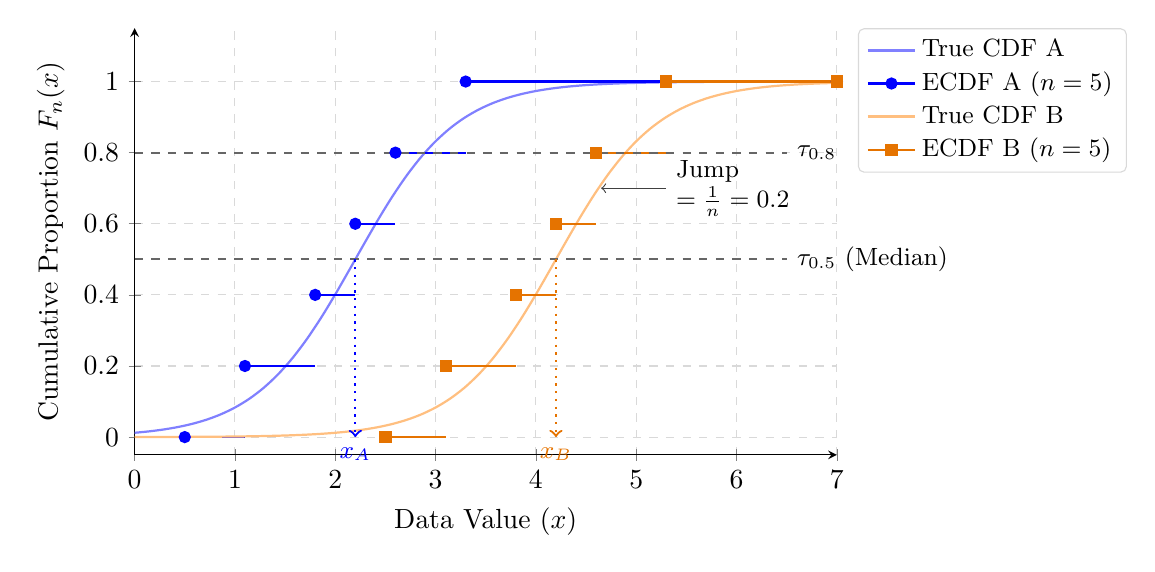
\begin{tikzpicture}
    \begin{axis}[
        width=10.5cm,
        height=7cm,
        xlabel={Data Value ($x$)},
        ylabel={Cumulative Proportion $F_n(x)$},
        xmin=0, xmax=7,
        ymin=-0.05, ymax=1.15,
        xtick={0,1,2,3,4,5,6,7},
        ytick={0, 0.2, 0.4, 0.6, 0.8, 1.0},
        grid=major,
        grid style={dashed, gray!30},
        axis lines=left,
        % Legend placed outside the plot to the right
        legend pos=outer north east,
        legend style={font=\small, cells={anchor=west}, draw=gray!30, rounded corners=2pt},
        clip=false % Allows labels outside the axis bounds to be visible
    ]

    % ==============================================
    % DISTRIBUTION A (Base)
    % ==============================================
    % True CDF A
    \addplot[blue!50, smooth, thick, domain=0:7, samples=50] { 1 / (1 + exp(-2*(x-2.2))) };
    \addlegendentry{True CDF A};

    % ECDF A
    \addplot[blue, thick, const plot, mark=*, mark options={solid, scale=0.9}, jump mark left] coordinates {
        (0.5, 0)
        (1.1, 0.2)
        (1.8, 0.4)
        (2.2, 0.6)
        (2.6, 0.8)
        (3.3, 1.0)
        (7.0, 1.0)
    };
    \addlegendentry{ECDF A ($n=5$)};

    % ==============================================
    % DISTRIBUTION B (Shifted)
    % ==============================================
    % True CDF B
    \addplot[orange!50, smooth, thick, domain=0:7, samples=50] { 1 / (1 + exp(-2*(x-4.2))) };
    \addlegendentry{True CDF B};

    % ECDF B
    \addplot[orange!90!black, thick, const plot, mark=square*, mark options={solid, scale=0.9}, jump mark left] coordinates {
        (2.5, 0)
        (3.1, 0.2)
        (3.8, 0.4)
        (4.2, 0.6)
        (4.6, 0.8)
        (5.3, 1.0)
        (7.0, 1.0)
    };
    \addlegendentry{ECDF B ($n=5$)};

    % ==============================================
    % THRESHOLDS & ANNOTATIONS (\tau)
    % ==============================================
    
    % Threshold: Tau = 0.5 (Median)
    \draw[dashed, black!60, thick] (axis cs:0, 0.5) -- (axis cs: 6.5, 0.5) 
        node[right, font=\small, text=black] {$\tau_{0.5}$ (Median)};
    
    % Dropdown markers showing where Tau=0.5 intersects the ECDFs
    \draw[dotted, blue, thick, ->] (axis cs:2.2, 0.5) -- (axis cs:2.2, 0) 
        node[below, font=\small] {$x_A$};
    \draw[dotted, orange!90!black, thick, ->] (axis cs:4.2, 0.5) -- (axis cs:4.2, 0) 
        node[below, font=\small] {$x_B$};

    % Threshold: Tau = 0.8
    \draw[dashed, black!60, thick] (axis cs:0, 0.8) -- (axis cs: 6.5, 0.8) 
        node[right, font=\small, text=black] {$\tau_{0.8}$};

    % Jump height explanation (moved to a clear spot on curve B)
    \draw[<-, darkgray] (axis cs:4.65, 0.7) -- (axis cs:5.3, 0.7) 
        node[right, font=\small, text=black, align=left] {Jump \\ $= \frac{1}{n} = 0.2$};

    \end{axis}
\end{tikzpicture}